\documentclass[twocolumn]{article}
\usepackage{graphicx} % Required for inserting images
\usepackage{biblatex}
\usepackage{textcomp}
\bibliography{references}

\title{Altium as an Electronic Design Automation Software for Smartfin}
\author{
  Josephine Dominguez\\
  UC Santa Cruz\\
  \texttt{jocadomi@ucsc.edu}
  \and
  Jordan Reichhardt\\
  Cal Poly San Luis Obispo\\
  \texttt{jreichha@calpoly.edu}
}

\date{August 2023}

\begin{document}

\maketitle

\section*{Abstract}
Altium is an Electronic Design Automation (EDA) software for developing Printed Circuit Boards (PCBs). Often heralded as the “industry standard”, Altium provides a multitude of features such as portability, version control, and design rule parameters to improve workflow in PCB design, but also has pitfalls in cost and high processing requirements. Due to the future obsoletion of Autodesk Eagle, UCSD Engineers for Exploration opted for Altium in summer research. The goal of this white paper is to examine the pros, cons, and process of using Altium in the creation of the Smartfin 3.0 PCB for future reference.

\section{Connected Workspace and Version Control}
Altium functions off of an integrated Git version control system which works in tandem with its Connected Workspace. Altium users can create and join servers for their institution or company, enabling all members to share projects and update components to a joint library. Additionally, the Git repository allows users to commit and push files and components. The History and Version control tab, which can be accessed on any file in a project, is used to observe branching and resolve conflicts. 

Throughout the development of the Smartfin 3.0 PCB, we utilized this version control system seeing as we had multiple contributors to one PCB. Conflicts were easily resolved and the shared library system streamlined our process.

\section{Library Reconstruction}

Components in Altium consist of a footprint and schematic symbol. The footprint is crucial for the board design because it dictates the size and shape of electronically-conductive pads; a physical component will be propagated on the pads and thus on the board. The schematic aspect of components is important for the designer or viewer of the PCB design because it illustrates electronic symbols and circuit layout. 

\begin{figure}[h]
    \centering
    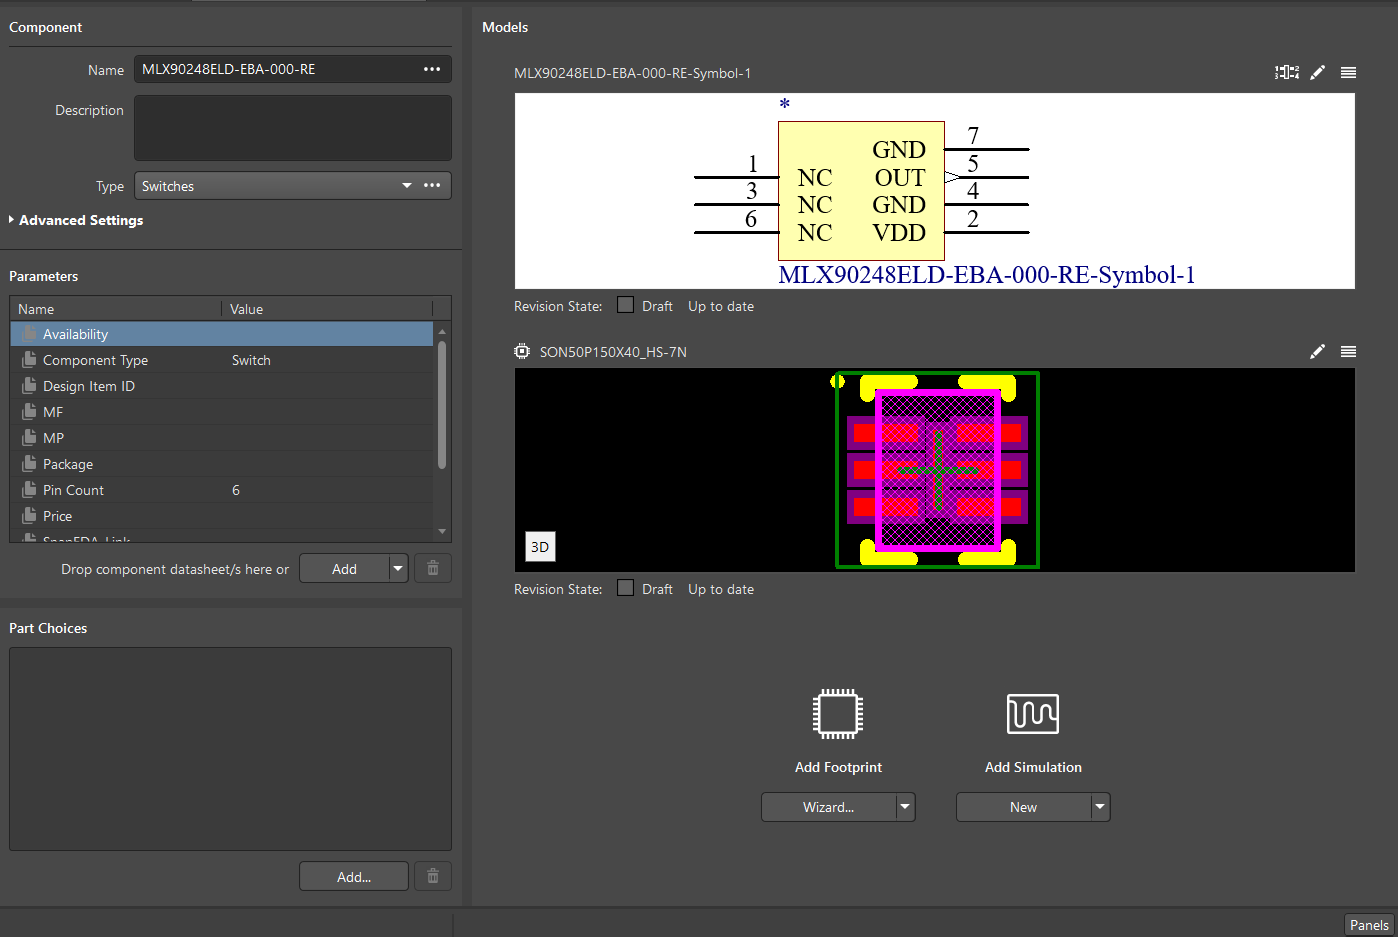
\includegraphics[width=0.4\textwidth]{component example.png}
    \caption{Schematic symbol and footprint in Altium component editor}
    \label{fig:component-editor}
\end{figure}

\subsection{Sourcing}
At the beginning of summer research, resources for the Smartfin PCB consisted of an Altium schematic file, board file, Bill of Materials (BOM), and manufacturing files. Unfortunately, the library (database for storing components in EDA software) was inaccessible to UCSD, rendering all components and their corresponding symbols and footprints unusable. Every component needed to be re-sourced from suppliers such as Digikey\cite{Digikey} and Mouser\cite{Mouser}. The component names were cross-checked with the BOM, and EDA source files were located. We used Snap EDA\cite{SnapEDA} files in re-sourcing the symbols and footprints, but Altium has scripting capabilities if Ultra Librarian\cite{UltraLibrarian} is preferred. Additionally, we utilized the built-in Altium Import Wizard to port the Snap EDA files into Altium and furthermore, onto the UCSD server. 

The sourcing of the Particle T-SoM symbol and footprint was especially difficult, but made possible by Altium’s accessibility features. The footprint was not in the Particle datasheet for the product, so manual construction was attempted, requiring the laying out of 100 individual pads with millimeters of accuracy. During this process, it was made known that the footprint was included in the TSoM eval board data sheet on a site external to the Particle site. 

\begin{figure}[h]
    \centering
    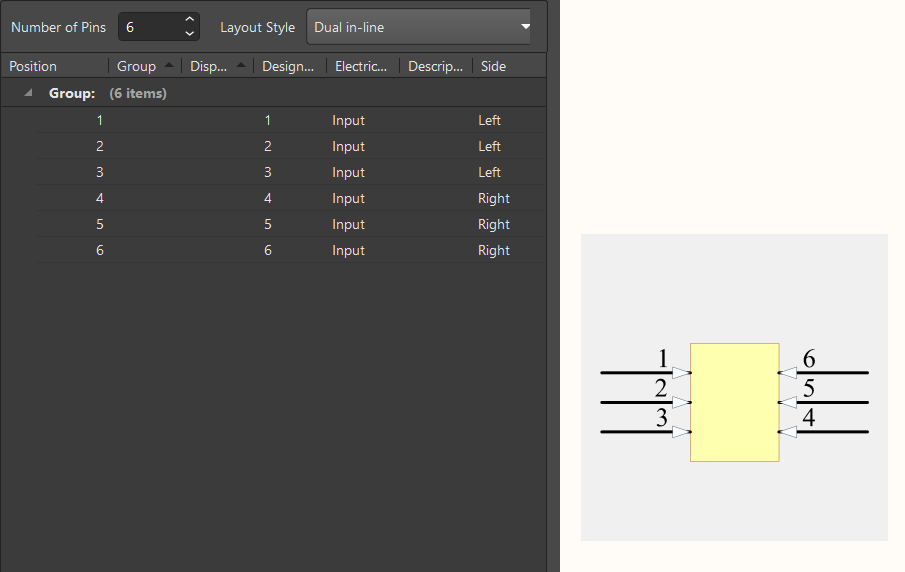
\includegraphics[width=0.4\textwidth]{symbol wizard.png}
    \caption{Symbol Wizard interface with pinout options}
    \label{fig:enter-label}
\end{figure}

The footprint was then copied off of the original board file from the PCB and pasted into the component editor. The symbol was generated using the Symbol Wizard which allows the user to map out pins and provide electrical characteristics, not only improving organization of schematics, but also enabling electrical simulation via software such as PSpice.

\subsection{Manually-Created Components}
All components unable to be sourced were recreated manually in the component editor using measurements found in their datasheets, and then updated to the shared UCSD server. The Altium Component Wizard greatly improved efficiency in creating Integrated Circuits (ICs) and Surface-Mounted Devices (SMDs), seeing as it provides templates for certain packaging and generates a corresponding footprint. 

\begin{figure}[h]
    \centering
    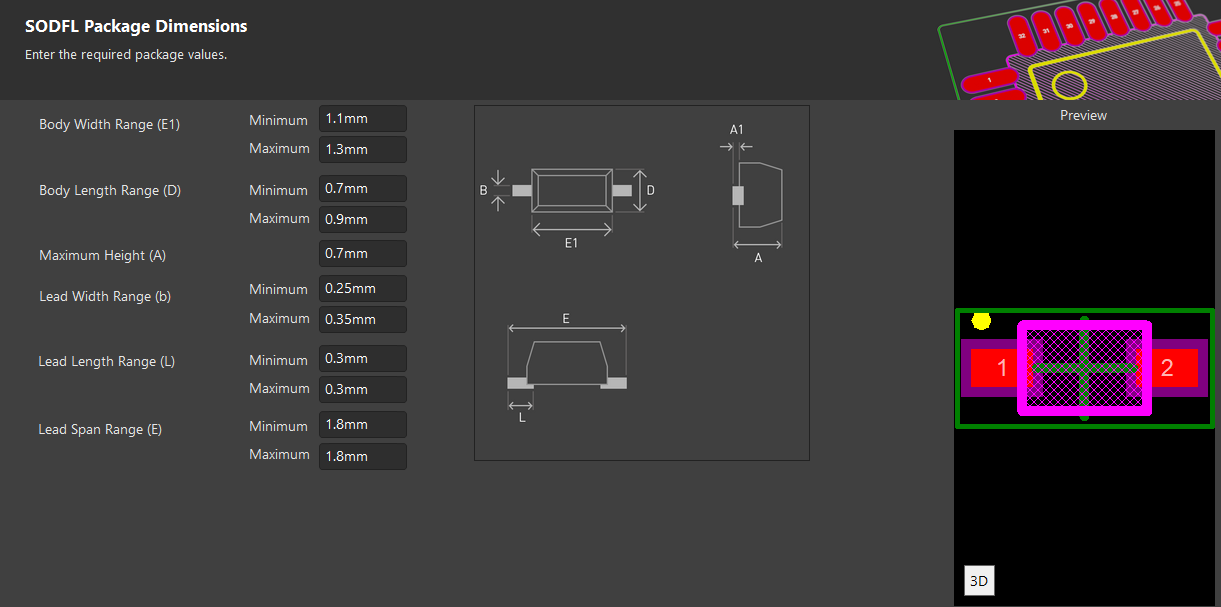
\includegraphics[width=0.4\textwidth]{component wizard.png}
    \caption{Component Wizard interface with size parameters}
    \label{fig:component-wizard}
\end{figure}

However, we found issues in some manually-created components and in the Altium editing interface. The robust parameter system found in Altium has both the benefit of making manufacturability streamlined but at the cost of finicky software, often producing errors that could only be troubleshooted by changing the “class” of the component (I.E. registering a fuse as an IC). These issues were mostly alleviated by restarting the program. Overall, the accessibility and component design features of Altium made the library reconstruction process feasible.

\section{Design Rules}

One of Altium's most prominent features is its Design Rule editor, containing a multitude of parameters and presets that a user may change based off of preference. While the PCB is open, Design Rules are accessed via Design \textgreater Rules.

It is imperative that Design Rules reflect the constraints of manufacturers. Prior to generating a PCB, most rules should be established and edited to improve workflow. 

\section{PCB Generation and Layout}

Before processing the schematics onto a board, an Altium user can run an Electronic Rule Check (ERC) to ensure the project is electronically sound, found in Project \textgreater Run ERC. This will check that all components are connected. All unconnected pins and symbols must be marked off with a Generic No ERC symbol, which appears as a red X and is found by right-clicking the Parameter Set icon on the toolbar. The ERC will generate a list of errors under the Messages tab, all of which can be clicked and direct a user to the error in question. 

\begin{figure}[h]
    \centering
    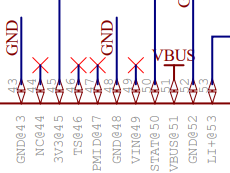
\includegraphics[width=0.3\textwidth]{noERC.png}
    \caption{Generic No ERC symbol added to unconnected pins}
    \label{fig:No-ERC}
\end{figure}

After all errors are resolved, the ERC should no longer appear under the Project tab, and the PCB can be generated through Design \textgreater Update PCB Document. The user then validates changes, and the PCB board file is created. Altium enables users to both update a PCB by editing the schematic, and update a schematic by editing the PCB, of which are found under the same Design \textgreater Update path. Once components are generated, they will be connected by “airwires”, or unrouted connections. Altium provides a unique and intuitive board layout software which automatically airwires to the nearest connection, streamlining the routing process. 

\subsection{Board Layout}
Aspects of board layout include placing capacitors near components they filter, high-speed connections such as USB, size of the board, accessibility of pads and connectors for testing and power, and any connections that are designed to be desoldered (i.e. 0 ohm resistors). Through-hole components will need to be easily accessible to solder to. Additionally, important considerations are power and ground planes, so providing ground-netted vias (drilled holes that carry traces from one layer of the board to another) and grouping components near their power source is crucial. Any component, pad, or via can be “netted”, or assigned to a specific electronic network. This is accessed under the Properties panel, or by right-clicking on any component in the board editor. 

Altium has three board views accessible by pressing “1”, “2”, or “3” on the keyboard. “1” is board planing view, which streamlines shaping the PCB. “2” is footprint view, the most important in board layout. “3” is 3D view, a generation of a 3D board and any component STEP files, enabling easy visualization. 

\begin{figure}[h]
    \centering
    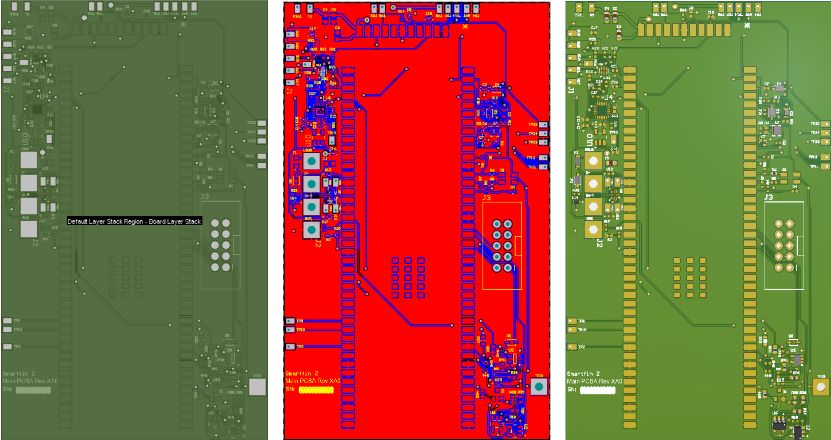
\includegraphics[width=0.3\textwidth]{board view.png}
    \caption{From left to right, board view "1", "2", and "3"}
    \label{fig:board-view}
\end{figure}

\section{Routing}

A critical step of PCB design is routing between components. Routing creates physical connections between components that will be printed as a copper trace when the PCB is fabricated. With simpler designs, users can run the Autoroute function, found under Route \textgreater Autoroute. This is when Altium automatically connects airwires between components. Unfortunately, with more complex designs such as the Smartfin PCB, Autorouting is often not a viable option as the PCB will end up with many airwires where autorouting failures occur.

\subsection{Vias}
Vias are crucial to the routing process, allowing traces that would otherwise overlap to bypass one another and avoid shorting. The Smartfin board has two layers, so vias were both necessary and reduced routing clutter. They were placed systematically to minimize the quantity, prevent crowding, and lower the overall cost of the board. Vias can also be used as heat sinks if there are any components that require heat management. 

\subsection{Trace Width}
Another aspect of routing is considering trace width. The Smartfin had three trace widths based on three general current ratings. The current ratings are for 30mA (data lines), 300mA (low power to components) and 1A (high power lines such as LIPO). These currents were put into a trace width calculator in order to produce the necessary width for routing to each of these components. The trace width settings are accessed in the Design Rules. 

\subsection{Differential Pairs}
Components that require data lines with differential pairs are an important consideration when routing. Differential pairs are two wires that have the same magnitude of voltage but an opposite polarity. The component the differential pairs are routed to takes the difference between the pairs 
and processes that data. 

\begin{figure}
    \centering
    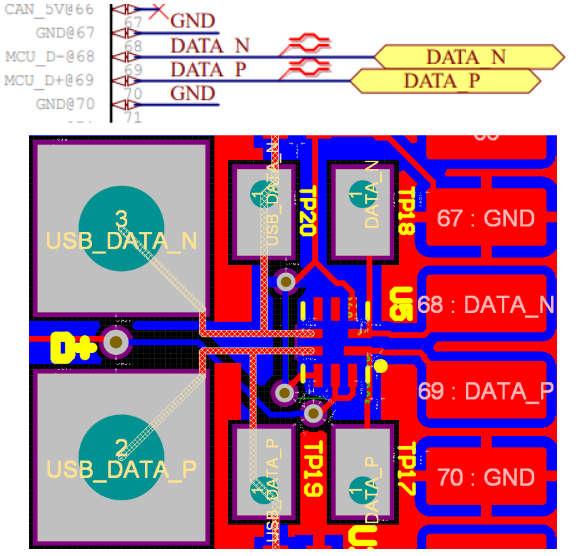
\includegraphics[width=0.3\textwidth]{differential pair.png}
    \caption{Differential pair designators on schematic and corresponding routed pair}
    \label{fig:differential-pair}
\end{figure}

For this reason, differential pair lines must be routed at exactly the same length so the receiving circuitry can properly analyze the difference between them. Altium possesses a differential pair tool which enables users to create wires of the same length and routed in parallel to one another. These pairs are specified on the schematic through Place \textgreater Directives \textgreater Differential Pairs, and to route, right-click the Routing icon in the PCB toolbar and select Interactive Differential Pair Routing. Differential Pair options are accessed in the Design Rules. 

\section{Design Rule Check and Manufacturing}

Throughout the routing process, Altium will flag errors in a board design. Most of these occur because of the proximity of components or traces to the edge of the board, to other traces, or to other components. Specific errors can be viewed through the Design Rule Check (DRC) under Tools \textgreater Design Rule Check \textgreater Run Design Rule Check. The page displays each of the specific errors within the PCB design. Clicking on an error will direct the user to the specific component or trace in question. Errors can be waived if they are not important to a user’s design or the PCB’s manufacturability. 

\begin{figure}[h]
    \centering
    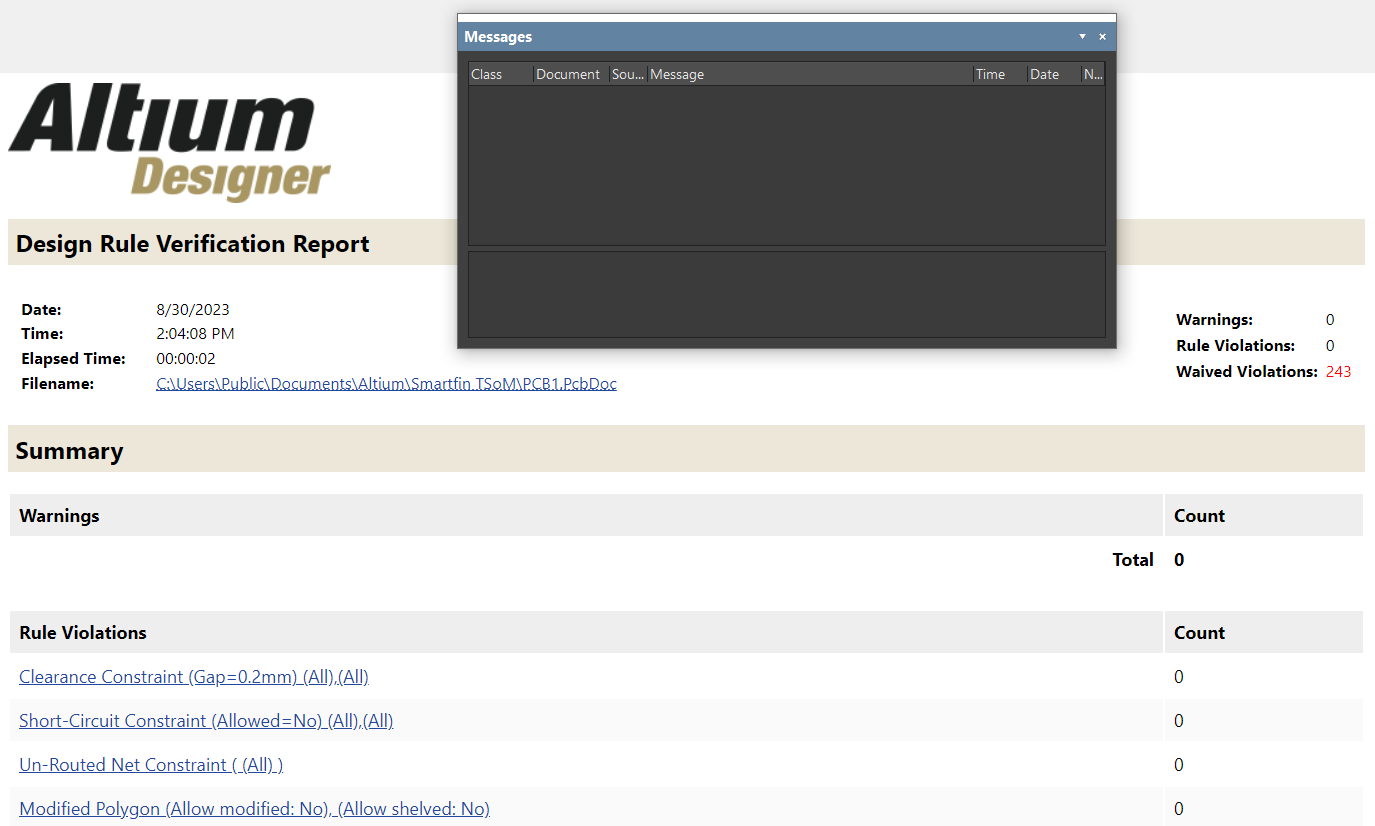
\includegraphics[width=0.4\textwidth]{DRC.png}
    \caption{Design Rule Check message panel and document}
    \label{fig:DRC}
\end{figure}

DRC violations are flagged because of certain parameters that are set under Design Rules. Some rules in this section were untouched in the process of creating the Smartfin 3.0, resulting in many errors needing to be waived by hand. 

\subsection{Fabrication}
In terms of manufacturability, Altium includes a multitude of export options. Under the File section, Altium provides Fabrication outputs containing everything from Drill Drawings to OBD++ zip files, all of which are imperative for board manufacturers. Additionally, Assembly Outputs generates drawings for future reference.

\subsection{Bill of Materials}
Altium also includes a built-in Bill of Materials (BOM) generator. Uploading an EDA file from a website such as Digikey will automatically include parameters such as manufacturer and pricing in the component editor and thus onto the BOM. When exporting the board to Macrofab\cite{Macrofab}, a PCB manufacturer, all components pre-sourced with EDA files included their corresponding part number and manufacturer, but manually-created components needed this information added individually. 

\section{Troubleshooting with Altium}

One major pitfall of Altium is the number of errors and issues a user may encounter during the EDA process. From constraint errors to “missing” files, the program Altium itself does not provide much assistance. Most troubleshooting was resolved using the Altium forum\cite{Altium}, followed closely by Stack Overflow\cite{StackOverflow} and Reddit\cite{Reddit}. Even with these resources, many issues were only solved through trial and error. A few errors unaddressed by the internet are as followed:

\begin{itemize} 
\item {In the symbol section of the component editor, only one end of a pin is considered “electronically conductive” by Altium’s ERC. Multiple manually-created components had their pins reversed, rendering them non-conductive, and thus producing errors. Flipping these pins in the component editor so the ends with cursors pointed outward alleviated this issue.}
 
\item {When generating an OBD++ file, Altium generates an error and a blank CAM file. The file cannot be found on the software itself, and is instead in file path This PC \textgreater Local Disk \textgreater Users \textgreater Public \textgreater Public Documents \textgreater Altium \textgreater “Project Name” \textgreater Project Outputs for “Project Name”. The file path however can be changed in Altium under Projects and Project Output.}

\item {If you generate a project from outside of your workspace and do not have the project’s library, the component footprints will not exist, nor can you copy them to new replacement components. All must be re-sourced and replaced in order to properly generate a PCB.}

\item {Forums severely undermine the importance of the Design Rules section of Altium, where multiple parameters can be set to improve the efficiency of EDA. Trace width, via size, differential routing, and many more features can be added and edited. This was especially important when laying out the PCB.}

\end{itemize}

The lack of accessible documentation slowed the EDA process down and was the main contributor to the stagnation of progress. However, most issues were resolved by cross-checking forums and researching corresponding videos. 


\section{Conclusion}

Altium as an EDA software in the creation of the Smartfin 3.0 proved to improve workflow efficiency through integrated version control, robust parameter options, and intuitive import and export features. Furthermore, errors encountered during the process, albeit difficult to troubleshoot, eventually were resolved using resources such as forums and videos. This white paper serves as a document for future use of Altium in UCSD E4E to alleviate these roadblocks.

\printbibliography

\end{document}

